\chapter{Thin strip graphs}
\label{chap:thinDef}

The goal of this chapter is to introduce you to the main subject of this thesis. Thin strip graphs is a class of graphs that lay between unit disk graphs
and mixed interval graphs. We can define formally a $c$-strip graph as a unit disk graph such that the centers of the disks belong to $\{(x,y) : -\infty < x < \infty, 0 \leq y \leq c\}$, more intuitively we can see this as a unit disk graph where the centers of the disks lay between two parallel horizontal lines with a distance of $c$ between them. We denote this class by SG($c$). We
have then that SG($0$) = UIG and SG($\infty$) = UDG.

The definition and main work for this class comes from Breu in his thesis \cite{breuAlgorithmicAspectsConstrained1996}. However, Hayashi et al. \cite{hayashiThinStripGraphs2017} expand his work by defining the class of \emph{thin strip graphs}.

\section{Thin strip graphs}

A thin strip graph can be intuitively defined as a $c$-strip graph where $c$ is an arbitrarily little $\varepsilon$. Also, we can see that SG($k$) $\subseteq$ SG($l$) with $k<l$. A more strict definition emerges from this observation:

\begin{defn}
  Thin strip graphs are defined as TSG $= \bigcap_{c > 0}$ SG($c$).
\end{defn}

\begin{remark}
  SG($0$) $\neq$ TSG. We can construct a $K_{1,3}$ such that we have 3 vertices with the coordinates
  $(1,0)$, $(0,0)$, $(1,0)$ and a last one $(0,\varepsilon)$ with $\varepsilon > 0$ and arbitrarily small
  as seen in Figure \ref{fig:thinK13}.
\end{remark}

% Figure about the K_1,3 construction
\begin{figure}
\centering

\begin{scaletikzpicturetowidth}{\textwidth}
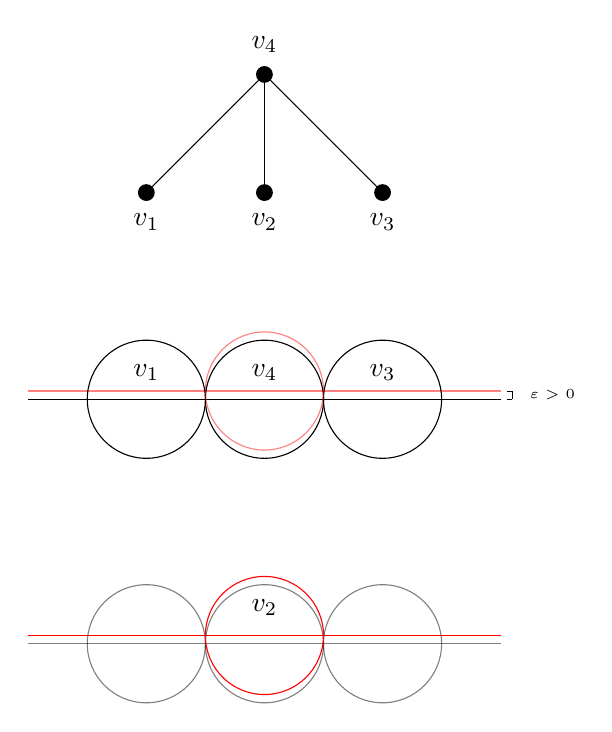
\begin{tikzpicture}[scale=1.5]

\draw (-2,0) -- (2,0);
\draw[red ,opacity = 0.5] (-2,0.07) -- (2,0.07);
\draw  (-1,0) circle [radius=0.5];
\draw[color=black] (-1,0.2265) node {$v_1$};
\draw  (0,0) circle [radius=0.5];
\draw[color=black] (0,0.2265) node {$v_4$};
\draw  (1,0) circle [radius=0.5];
\draw[color=black] (1,0.2265) node {$v_3$};

\draw[red, opacity = 0.5] (0,0.07) circle [radius=0.5];
\draw[color=black] (2.4386,0.0367) node {\tiny $\varepsilon > 0$};

% lines to describe distance (epsilon)
\draw[very thin] (2.1,0.07) -- (2.1,0);
\draw[very thin] (2.05,0.07) -- (2.1,0.07);
\draw[very thin] (2.05,0) -- (2.1,0);

\draw[opacity = 0.5] (-2,-2.07) -- (2,-2.07);
\draw[red] (-2,-2) -- (2,-2);
\draw[opacity = 0.5]  (0,-2.07) circle [radius=0.5];
\draw[opacity = 0.5]  (1,-2.07) circle [radius=0.5];
\draw[opacity = 0.5]  (-1,-2.07) circle [radius=0.5];
\draw[red] (0,-2) circle [radius=0.5];
\draw[color=black] (0,-1.765) node {$v_2$};

\node[draw,circle,inner sep=2pt,fill,label distance=1cm] (v1) at (0,2.75) {};
\draw[color=black] (0,3) node {$v_4$};
\node[draw,circle,inner sep=2pt,fill,label distance=1cm] (v3) at (0,1.75) {};
\draw[color=black] (0,1.5) node {$v_2$};
\node[draw,circle,inner sep=2pt,fill,label distance=1cm] (v2) at (-1,1.75) {};
\draw[color=black] (1,1.5) node {$v_3$};
\node[draw,circle,inner sep=2pt,fill,label distance=1cm] (v4) at (1,1.75) {};
\draw[color=black] (-1,1.5) node {$v_1$};
\draw  (v1) edge (v2);
\draw  (v1) edge (v3);
\draw  (v1) edge (v4);
\end{tikzpicture}
\end{scaletikzpicturetowidth}
\caption{A construction of $K_{1,3}$ with a disk realization, being this graph a TSG.}
\label{fig:thinK13}
\end{figure}

\begin{theorem}[Hayashi et al. \cite{hayashiThinStripGraphs2017}]
  There is no constant $t$ such that SG($t$) = TSG.
\end{theorem}

\begin{theorem}[Hayashi et al. \cite{hayashiThinStripGraphs2017}]
  There is no constant $t$ such that SG($t$) = UDG.
\end{theorem}

Hayashi et al. left some open problems. I try to expand the knowledge around some of these problems
to help the understanding of them, largely the recognition of this class of graphs. Before, we see where this class lays in the hierarchy of classes. We know by definition that TSG $\subsetneq$ UDG.

\subsection{Interval graphs}

Thin strip graphs shares their geometrical structure with interval graphs (remember SG($0$) = UIG). In this subsection, we overview the results of Hayashi et al. \cite{hayashiThinStripGraphs2017} where they find maximal and minimal superclasses for TSG in the interval graphs presented in chapter \ref{chap:interval}. The following theorem will be proven by taking the proof written by Hayashi et al. in order to use their mapping in other theorems (e.g. \ref{chap:twolevel}).

\begin{theorem}[Hayashi et al. \cite{hayashiThinStripGraphs2017}]
  MUIG $\subsetneq$ TSG.
\end{theorem}

\proof{
First, we prove that MUIG $\neq$ TSG. This can be proven because $C_4 \in$ TSG if we take as points $(0,0),(0,\varepsilon),(1,0),(1,\varepsilon)$ with $1 >\varepsilon > 0$ and $C_4 \notin$ MUIG because it is a chordal graph.

Then, we have to prove that MUIG $\subseteq$ TSG. Let $G = (V,E) \in$ MUIG where each vertex is a unit mixed interval denoted as $I_v$. We define $t = \min\{|I_u\cap I_v| : |I_u\cap I_v| > 0, \{I_u,I_v\} \subseteq V\}$ and $s = \min\{\ell(I_v) - r(I_u) : \ell(I_v) > r(I_u), \{I_u,I_v\} \subseteq V\}$. We have then $t$ being the minimum length of an intersection bigger than zero (that is, not endpoint-adjacent) and $s$ is the minimum distance between non-adjacent vertices (also not endpoint-adjacent). We also define $c(I_v) = \frac{\ell(I_v) + r(I_v)}{2}$ as the center of the interval and $p(I_v) = (-1)^{\left \lfloor{c(I_v)}\right \rfloor }$.

Let $d$ be a real such that $0 < d < \frac{2}{3}$, $d\leq \frac{t}{4}$, $d < \frac{s}{2}$ and $\varepsilon \geq 2\sqrt{d-d^2}$. If we let $h = \sqrt{d-d^2}$, then we can create a $2h$-realization of $G$ with the following mapping:

\[ \phi(v) =
  \begin{cases}
      (c(I_v),0) & \text{if}\  I_v\  \text{is a closed interval} \\
      (c(I_v),hp(I_v)) & \text{if}\  I_v\  \text{is an open interval} \\
      (c(I_v)-d,hp(I_v)) & \text{if}\  I_v\  \text{is a closed-open interval} \\
      (c(I_v)+d,hp(I_v)) & \text{if}\  I_v\  \text{is an open-closed interval}
   \end{cases}
\]

For two vertices $u$ and $v$ of $G$ such that $u < v$, we have the three following cases:

\begin{enumerate}
  \item $r(I_u) < \ell(I_v)$:

    $I_u$ and $I_v$ are not adjacents, which means that $\text{dist}(\phi(u),\phi(v)) > 1$.
    If we minimize the distance between them we have $\phi(u) = (c(I_v)+d,hp(I_v))$ and $\phi(v) = (c(I_v)-d,hp(I_v))$. Therefore,

    
  \item $r(I_u) > \ell(I_v)$:
  \item $r(I_u) = \ell(I_v)$:
\end{enumerate}
}

We can define a new class of graphs: unfettered unit interval graphs. These graphs
are unit interval graphs where if two intersections touch, we can decide whether
they intersect or not. We denote this class UUIG.

\begin{theorem}[Hayashi et al. \cite{hayashiThinStripGraphs2017}]
  TSG $\subsetneq$ UUIG.
\end{theorem}

\proof{See \cite{hayashiThinStripGraphs2017}.}

\todo{longer demonstration, maybe is going to go to the appendix.}


\section{Characterization of thin strip graphs}

One of the main goals of this thesis is to characterize TSG. by forbidden induced subgraphs. To approach this, we will see how many induced forbidden subgraphs are also forbidden for TSG. We have described the familes of forbidden induced subgraphs for MUIG in section \ref{sec:muig} and one of these familes has been proven to be a forbidden induced subgraph for TSG:

\begin{theorem}[Hayashi et al. \cite{hayashiThinStripGraphs2017}]
  $\mathcal{R}$ is a forbidden induced subgraph family of TSG.
\end{theorem}

\begin{figure}
\centering

\begin{scaletikzpicturetowidth}{\textwidth}
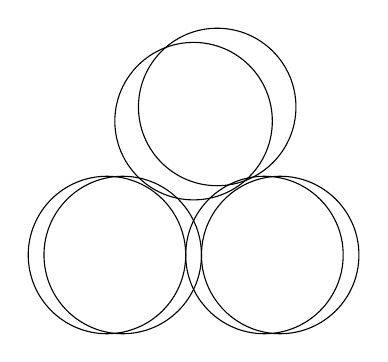
\begin{tikzpicture}[scale=2]

% line
\draw  (0,0) circle [radius=0.5];
\draw  (0.1,0) circle [radius=0.5];
\draw  (1,0) circle [radius=0.5];
\draw  (1.1,0) circle [radius=0.5];

%upper
\draw  (0.55,0.85) circle [radius=0.5];
\draw  (0.7,0.94) circle [radius=0.5];


\end{tikzpicture}
\end{scaletikzpicturetowidth}

\caption{A construction of $F$ with a unit disk realization.}
\label{fig:fUDG}
\end{figure}


With the properties presented in this chapter, we can begin to state our first hypothesis:

\begin{hyp}
  $F \in (\text{UDG}\cap\text{UUIG}) \setminus \text{TSG}$.
\end{hyp}

\begin{claim}
 $F \in (\text{UDG}\cap\text{UUIG})$
\end{claim}

\begin{proof}
  We can see that $F \in$ UDG because we can have a unit disk realization (Figure \ref{fig:fUDG}) and also has a level structure $L = \{K_2, K_3, K_1\}$.
\end{proof}

\begin{theorem}
$F \notin$ TSG.
\end{theorem}

\todo{this is bullshit, F is in fact in TSG...}

\proof{

The distance between $a$ and $d$ has to be at most 2, because there is at least one vertex that is adjacent to both. And clearly, the other points have to be between them because they are adjacent to both, so if they were not.
}

\section{Recognition}

The recognition of this class of graphs is stated by Breu in his thesis \todo{explain everything about dangerous cycles and
complement oriented graphs in Breu's paper}.
